\documentclass[10pt,twocolumn]{article}
\usepackage{geometry}
\geometry{verbose,headsep=3cm,tmargin=2.5cm,bmargin=2.5cm,lmargin=2.0cm,rmargin=2.0cm}
\usepackage{graphicx}
\usepackage{xcolor}
\usepackage[font=small]{caption}
\usepackage{amsmath,amssymb,latexsym}
\usepackage{marvosym}
\usepackage{url}
\usepackage{lipsum}
\usepackage{bm}
\usepackage{float}
\usepackage[english]{babel}
\usepackage{hyperref}
\usepackage{epsf}
\usepackage{float}
\usepackage{mathpazo}
\usepackage{pifont}
\usepackage{wrapfig}
\usepackage{multicol}
\usepackage{enumitem}
\usepackage{xcolor}
\usepackage{framed}
\usepackage[utf8]{inputenc}
\graphicspath{{DWGs/}}
\usepackage{framed}
\usepackage{textcomp}

% Document font:
\usepackage{charter}

\newcommand{\highlight}[1]{%
  \colorbox{orange!50}{$\displaystyle#1$}}

\begin{document}

%%% HEADER --------------------------------------------------------------
% ------------------------------------------------------------------------

\twocolumn[{
\begin{@twocolumnfalse}

  \begin{center}
%\textcolor{lgray}
    \vskip-5em

    \hfill
    \fontsize{10}{10}\selectfont {\textit{Bruxelles, December 2018}}
    \vskip2ex
	\vspace{5ex}
    \fontsize{24}{10}\selectfont {Notes on Principal Component Analysis}
      \vspace{1ex}
  \noindent%
    
\vskip1ex

{\rule{\textwidth}{0.5pt}}

  \end{center}
  
\vspace{8mm}

\end{@twocolumnfalse}
}]

%%% HEADER END -----------------------------------------------------------
% ------------------------------------------------------------------------

\vspace{10mm}

\setlength{\parindent}{0cm}

\fontsize{14}{10}\selectfont {Kamila Zdybał}

\vspace{2mm}

\fontsize{8}{10}\selectfont {\textit{Université libre de Bruxelles, kamila.zdybal@ulb.ac.be}}

\fontsize{8}{10}\selectfont {\textit{camillejr.github.io/science-docs, kamila.zdybal@gmail.com}}

\section*{Preface}

These are notes on \textbf{Principal Component Analysis} (PCA), a dimensionality reduction technique in which the data set is reduced to maintain only the directions of the largest variance.

\,\,

The deep and intuitive understanding of PCA requires the deep and intuitive understanding of basic linear algebra. I highly recommend a very pleasant to watch course by 3Blue1Brown YouTube channel, which, to my belief, will be everything you need to master about linear algebra to gain a great intuition behind PCA.

\,\,

This document is still in preparation. Please feel free to contact me with any suggestions, corrections or comments.

\section*{Keywords}

\textit{principal component analysis, data reduction, dimensionality reduction, linear algebra, MATLAB\textregistered, Python}

\tableofcontents

\section{Motivation for data reduction}

There are several questions which stimulated the usage of data reduction and data decomposition techniques:

\begin{enumerate}
\item Can we send less data but preserve maximum information contained by the data (data compression)?

\item If the data were measurements from an experiment, can we predict what the outcome of another measurement will be?

\item Can we build a model that will make predictions about a system?

\item Can we make sense of a large data set with high-dimensionality (which cannot be plotted graphically)?
\end{enumerate}

\section{Datasets for PCA}

For the rest of this document, we assume that the dataset for performing PCA is structured as follows: each column represents one variable $\text{Var}_j$ and the rows correspond to variable observations $\text{Obs}_i$ (e.g. at different positions in space, or in time).

\begin{figure}[H]
\centering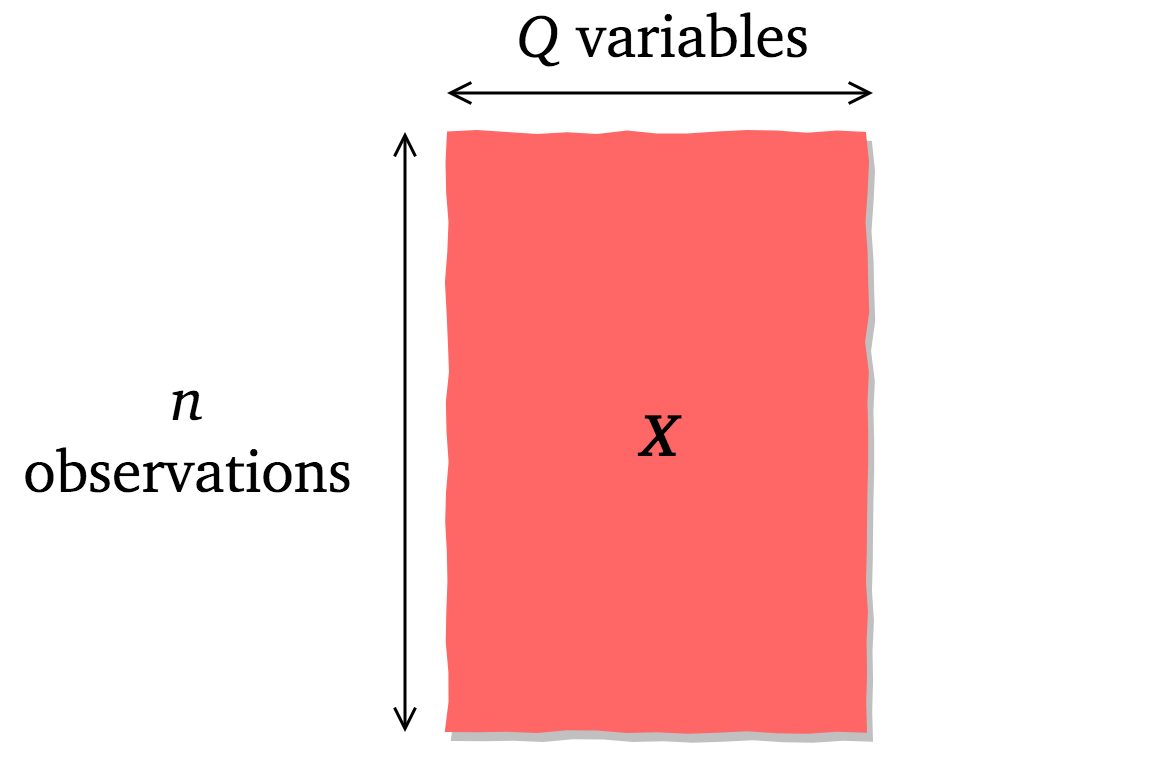
\includegraphics[width=5cm]{data-set-PCA.png}
\caption{Data matrix for PCA.}
\label{fig:data-matrix}
\end{figure}

This is also the data format that is needed for the MATLAB\textregistered \, command \texttt{pca}. From the documentation \cite{Matlab-pca}:


\begin{framed}
\texttt{pca(X)}
\,\,
Rows of X correspond to observations and columns correspond to variables.
\end{framed}

\section{Data pre-processing}

In data science we are typically given a raw data set which is not centered and not scaled. 

\section{Covariance matrix}

We start our discussion of PCA with explaining the concept of a \textit{covariance matrix}, since computing this matrix is a starting point for performing PCA. The covariance matrix is given by:

\begin{equation}
\bm{S} = \frac{1}{n-1} \bm{X}^T \bm{X}
\end{equation}

The covariance matrix $\bm{S}$ is therefore size $(Q \times Q)$.

We will start with exploring the meaning of $\bm{X}^T \bm{X}$. Let's look at the graphical representation of this matrix multiplication in Fig. \ref{fig:covariance-matrix}.

\begin{figure}[H]
\centering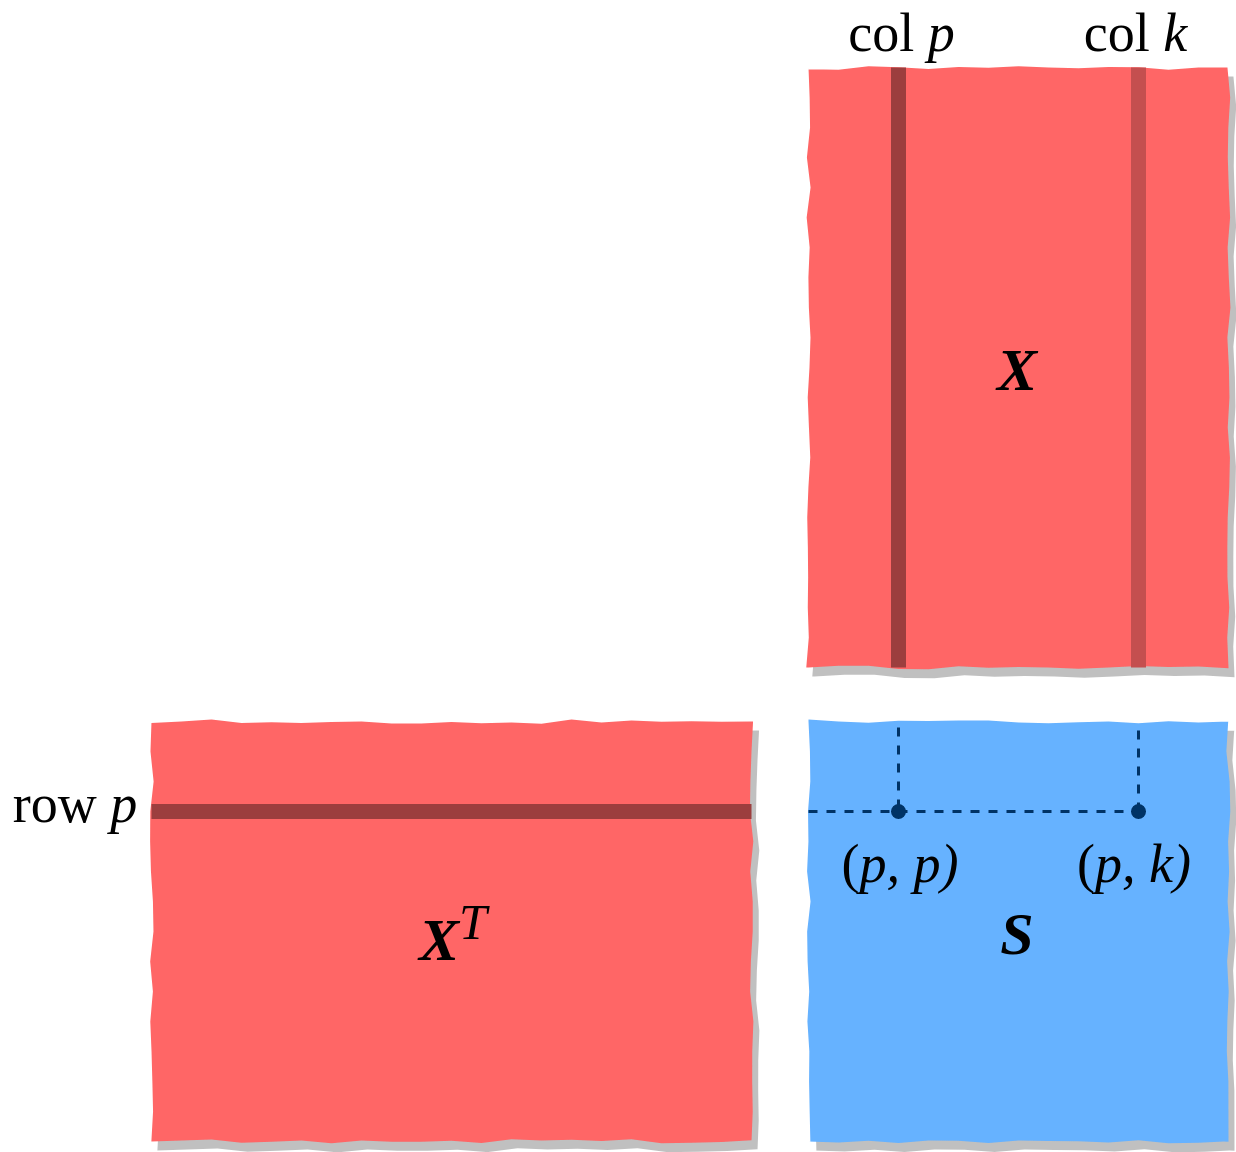
\includegraphics[width=7.5cm]{cov-matrix.png}
\caption{Covariance matrix $\bm{S}$ graphical interpretation.}
\label{fig:covariance-matrix}
\end{figure}

Any given column, say $p$ or $k$, of the data matrix $\bm{X}$ represents all measurements of a single variable $\text{Var}_p$ (or $\text{Var}_k$) and can be viewed as a single $n$-dimensional vector. The same can be said about any row of a matrix $\bm{X}^T$.

Notice that an element at position $(p,k)$ inside the matrix $\bm{S}$ has the interpretation of a dot product between a vector formed by the $p$-th row of a matrix $\bm{X}^T$ and a $k$-th column of a matrix $\bm{X}$. There is also the $\frac{1}{n-1}$ factor out front to which we will come back later.

\begin{equation}
s(p,k) = \frac{1}{n-1} dot( \bm{X}^T(p, :), \bm{X}(:,k))
\end{equation}

In a special case, where we multiply the row $p$ with the column $p$, we get a dot product of a vector with itself.

\begin{equation}
s(p,p) = \frac{1}{n-1} dot( \bm{X}^T(p, :), \bm{X}(:,p))
\end{equation}

In general, the dot product between two vectors $x$ and $y$ represents how much vector $x$ lays in the direction of vector $y$ (and vice versa) - and it is zero when two vectors are perpendicular to each other. This intuition can be carried to our covariance matrix $\bm{S}$. If any off-diagonal element is non-zero, say element at position $(p,k)$ this means that some information about variable $\text{Var}_p$ is carried by a variable $\text{Var}_k$ (and vice versa).

In other words, every element in the covariance matrix is:

\begin{equation}
s(i,j) = \frac{1}{n-1} \sum\limits_{k=1}^n \text{Var}_i(k) \text{Var}_j(k)
\end{equation}

\textbf{The goal of PCA in terms of a covariance matrix}

\,\,
\,\,

Principal Component Analysis aims to find a new, transformed data set $\bm{Z}$ such that if we computed a new covariance matrix:

\begin{equation}
\bm{S}_Z =  \bm{Z^T} \bm{Z}
\end{equation}

the variances (the elements on the diagonal) are maximized and the covariances (the off-diagonal elements) are zero. This means that no more information about any column of $\bm{Z}$ is carried by any other column of $\bm{Z}$.

\begin{figure}[H]
\centering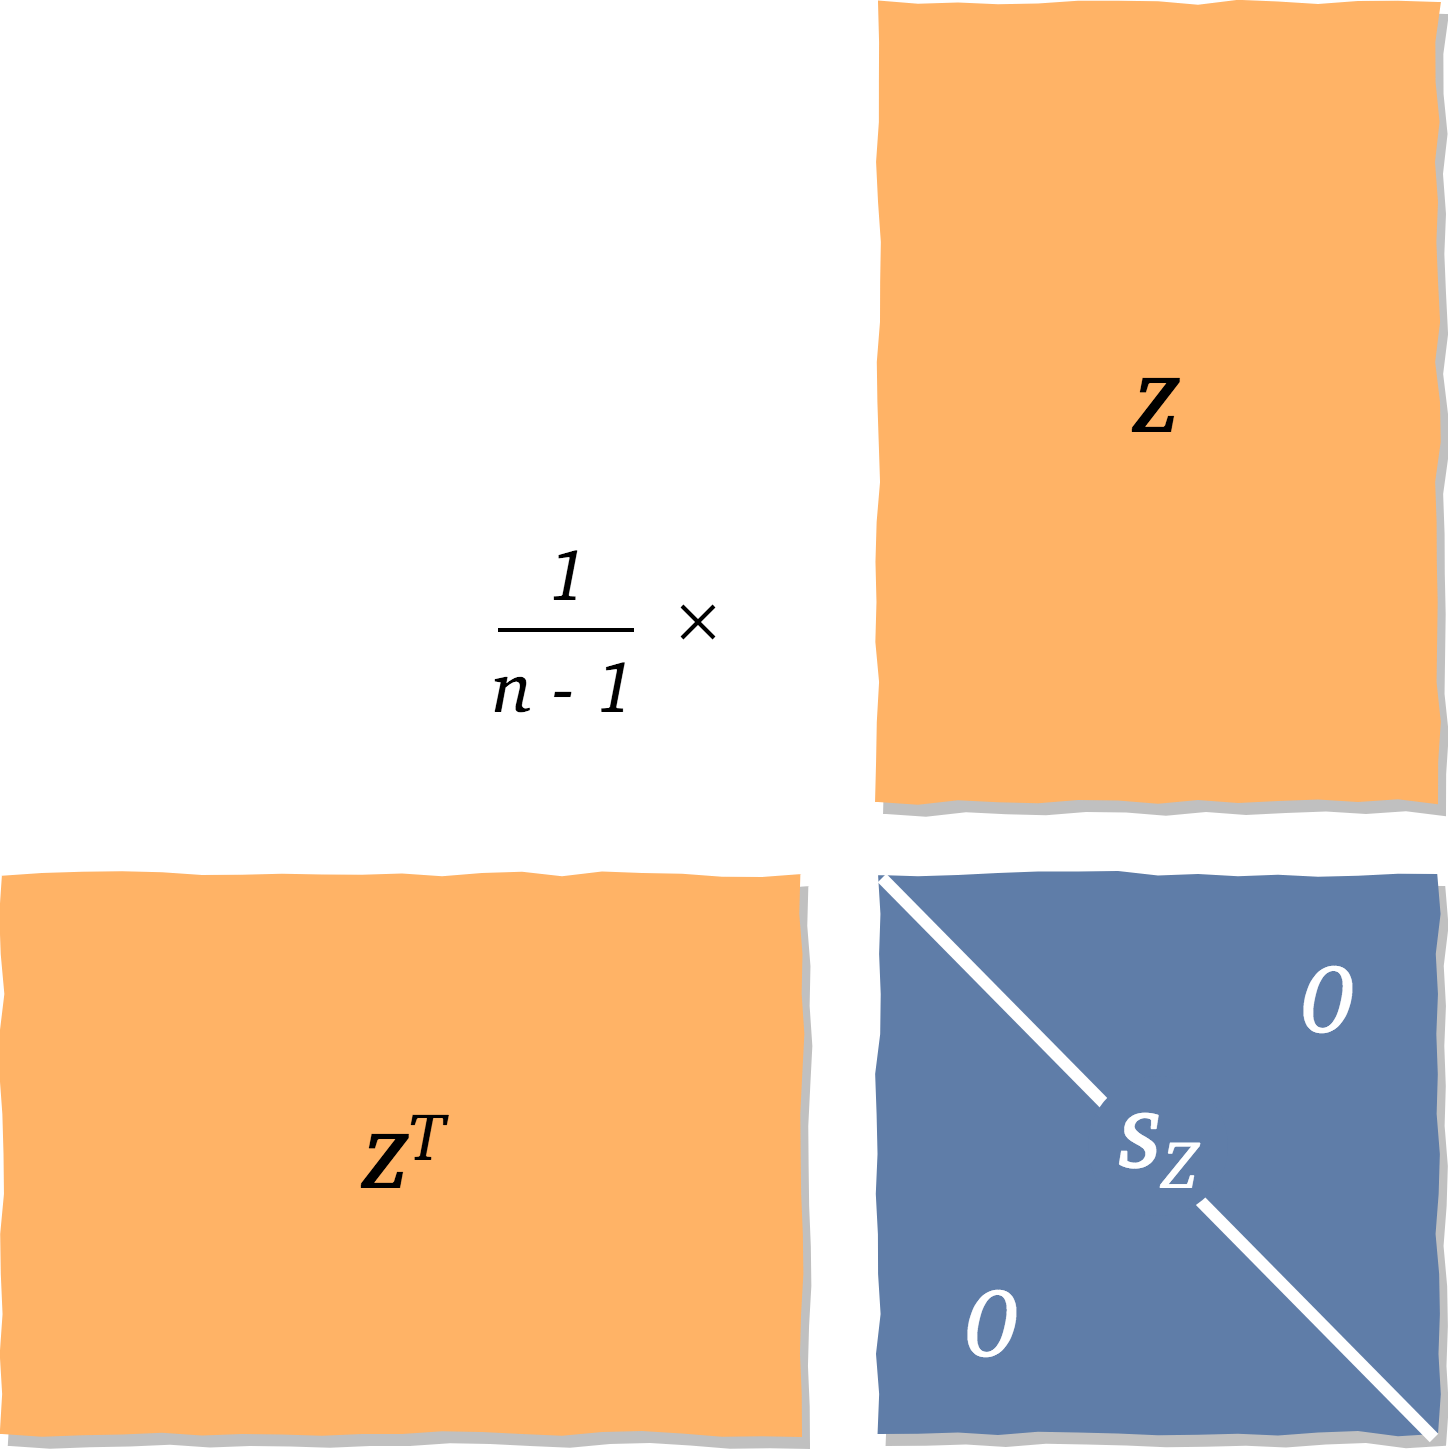
\includegraphics[width=6cm]{PC-scores.png}
\caption{New transformed data set $\bm{Z}$ and its covariance matrix $\bm{S}_Z$.}
\label{fig:PC-scores}
\end{figure}

\section{PCA workflow}

The next step in PCA is to perform the eigendecomposition of the covariance matrix:

\begin{equation} \label{eq:eig-dec}
\text{eig}(\bm{S}) = [\bm{A}, \bm{\Lambda}]
\end{equation}

The matrix $\bm{A}$ is a matrix of eigenvectors and it is size $(Q \times Q)$. Each eigenvector is called a \textit{principal component} (PC). The principal components are orthogonal to each other, and therefore the following important property holds: $\bm{A}^T = \bm{A}^{-1}$ (proof\footnote{Proof: for orthogonal columns of $\bm{A}$ we have $\bm{A}^T \bm{A} = \bm{I}$ Multiplying both sides by $\bm{A}^{-1}$ we get $(\bm{A}^T \bm{A}) \bm{A}^{-1}= \bm{I}\bm{A}^{-1}$. Since matrix multiplication is associative, we may also perform: $\bm{A}^T (\bm{A} \bm{A}^{-1}) = \bm{A}^{-1}$. From definition of an inverse matrix,  $\bm{A} \bm{A}^{-1} = \bm{I}$, hence: $\bm{A}^T = \bm{A}^{-1}$.}).

The diagonal matrix $\bm{\Lambda}$ of size $(Q \times Q)$ is a matrix of corresponding eigenvalues.

Given the eigendecomposition of matrix $\bm{S}$, we may state that: $\bm{S} = \bm{A} \bm{\Lambda} \bm{A}^T$.

The principal components form a new basis in which we can represent our data set. We therefore perform a transformation of the original data matrix $\bm{X}$ from the original space to the new space represented by the PCs. This transformation is achieved by the following multiplication:

\begin{equation} \label{eq:data-transform}
\bm{Z} = \bm{X} \bm{A}
\end{equation}



The new matrix $\bm{Z}$ is still our dataset $\bm{X}$ but represented in the basis associated with the matrix $\bm{A}$. It is also called the PC-\textit{scores} matrix, since one may think of every element in this matrix as the "score" that the corresponding element in $\bm{X}$ gets when represented in the new coordinate system after transformation.

\begin{wrapfigure}{R}{0.2\textwidth}
\centering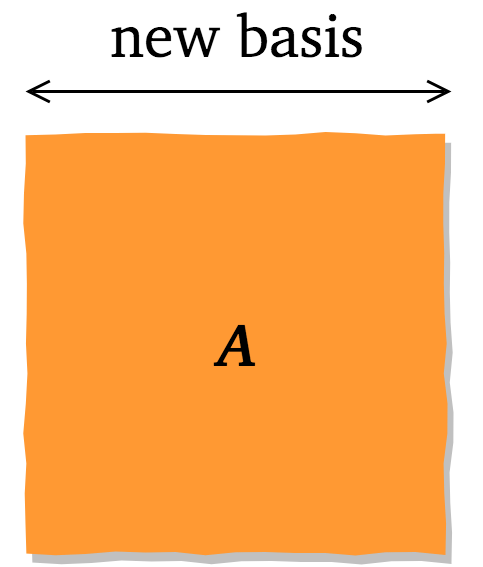
\includegraphics[width=3cm]{new-basis.png}
\caption{Eigenvalues of the covariance matrix form a new basis.}
\label{fig:new-basis}
\end{wrapfigure}


In the matrix multiplication from eq.(\ref{eq:data-transform}), every variable vector inside $\bm{X}$ gets transformed by the transformation matrix $\bm{A}$ and attains new scores in the basis associated with $\bm{A}$. The new representation of the old variable is now kept in the matrix $\bm{Z}$.

We now approach the dimensionality reduction but first let's obtain the original data set back, given the PC-scores and the transformation matrix:

\begin{equation}
\bm{X} = \bm{Z} \bm{A}^T
\end{equation}

The above equation is our route back to obtain the original data set in which the PC-scores are projected on the basis associated with a transposed eigenvectors matrix $\bm{A}$ (recall that $\bm{A}^T = \bm{A}^{-1}$).

Suppose that we would like to find the approximation of the data matrix $\bm{X}$ with only $q$ principal components (we project the PC-scores onto only $q$ out of $Q$ principal components).

We shrink the transformation matrix $\bm{A}$ to be of size $(Q \times q)$ (we only keep $q$ principal components). To match the matrix sizes we also need to shrink in size the PC-scores matrix which originally is size $(n \times Q)$ - the same size as the data matrix $\bm{X}$. We will denote these truncated matrices $\bm{A_q}$ and $\bm{Z_q}$ respectively.

Projecting $\bm{Z_q}$ onto the basis $\bm{A_q}^T$ will result in an an approximation of the original data set:

\begin{equation}
\bm{X_q} = \bm{Z_q} \bm{A_q}^T
\end{equation}


\begin{figure}[H]
\centering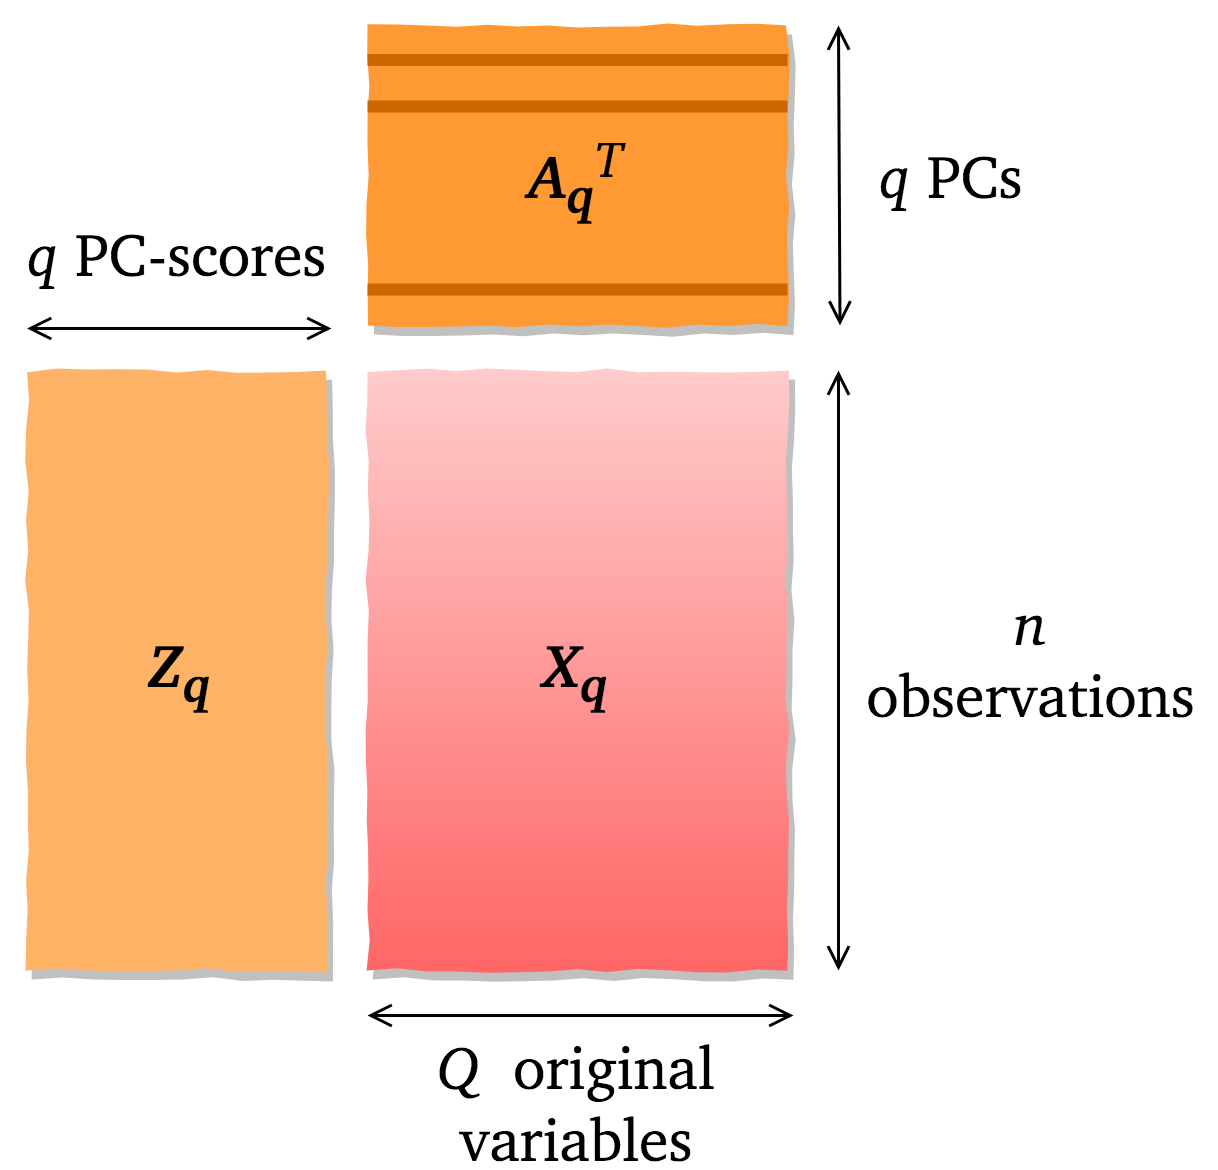
\includegraphics[width=7.5cm]{data-approx.png}
\caption{Data approximation with $q$-PCs.}
\label{fig:data-approx}
\end{figure}




\section{Why does it need to be eigenvectors?}

In this section we come back to equation (\ref{eq:eig-dec}) and answer the question: why are principal components the eigenvectors of a covariance matrix? If you are new to PCA, this indeed might seem like a not-related-to-anything thing to do. So why is it eigenvectors? And why does it need to be eigenvectors of this special matrix called covariance matrix?

To begin the understanding, let's look back at Figure \ref{fig:PC-scores}. What we want to achieve with PCA is to diagonalize the new covariance matrix. And we already have produced one diagonal matrix even before computing PC-scores - it was the matrix of eigenvalues $\bm{\Lambda}$.




\section{PCA Python example}

We will now go on to visualizing on a real 2D data set every step of PCA. We will use the PCA function from a Python library sklearn.decompositions. The full code can be accessed in the GitHub repository. Here, we will only recall elements of that code to explain what is happening.


\begin{figure}[H]
\centering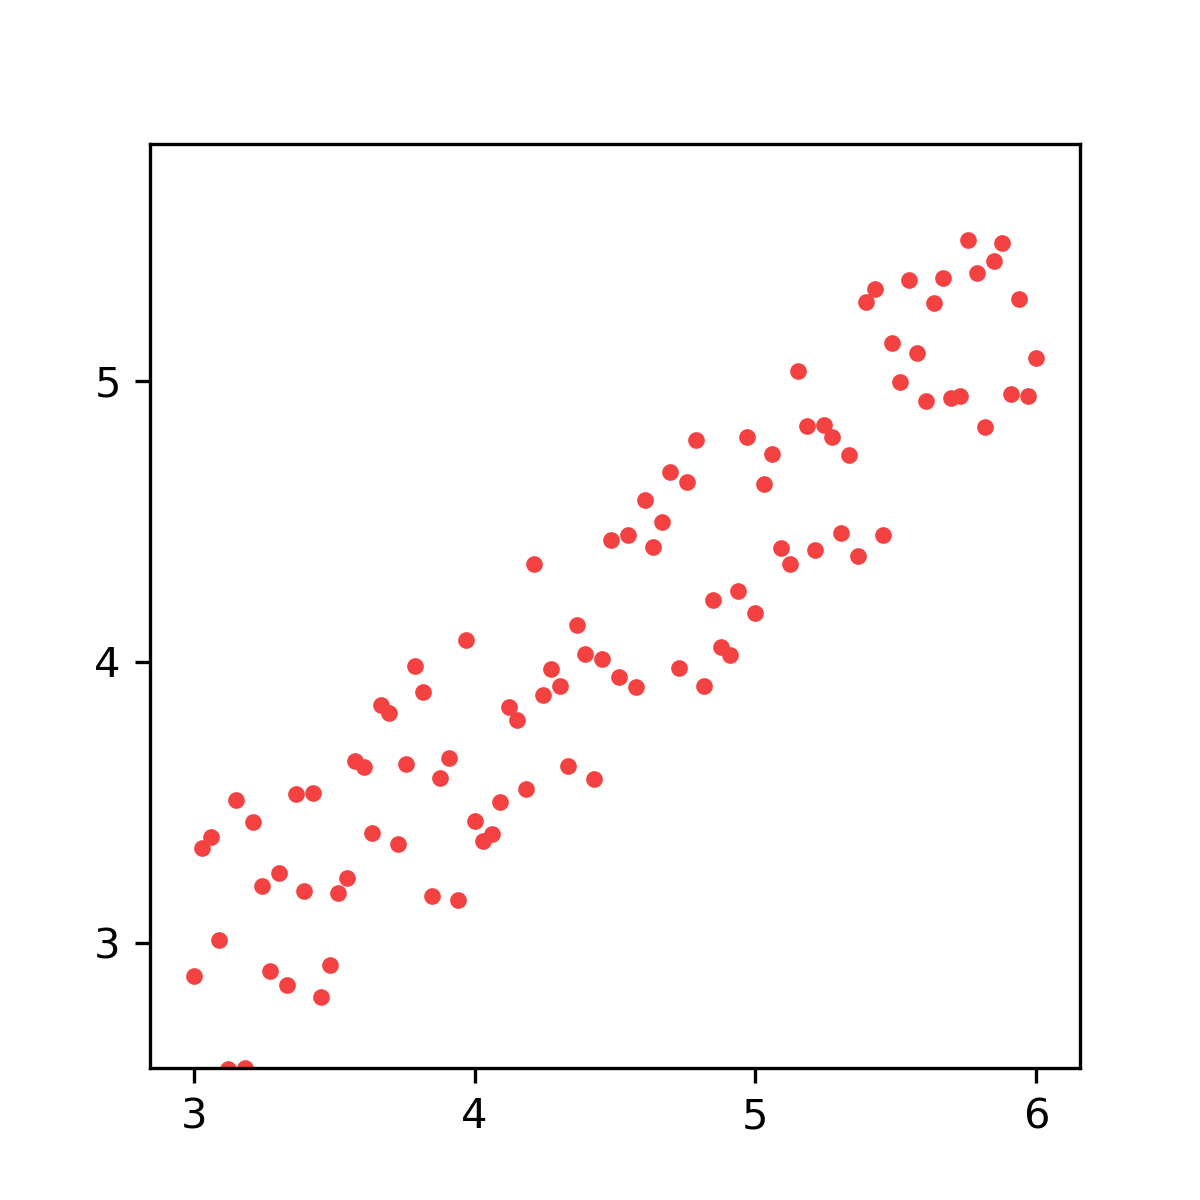
\includegraphics[width=7cm]{python-raw-data.png}
\caption{Raw dataset $\bm{X}$.}
\label{fig:python-raw-data}
\end{figure}

\begin{figure}[H]
\centering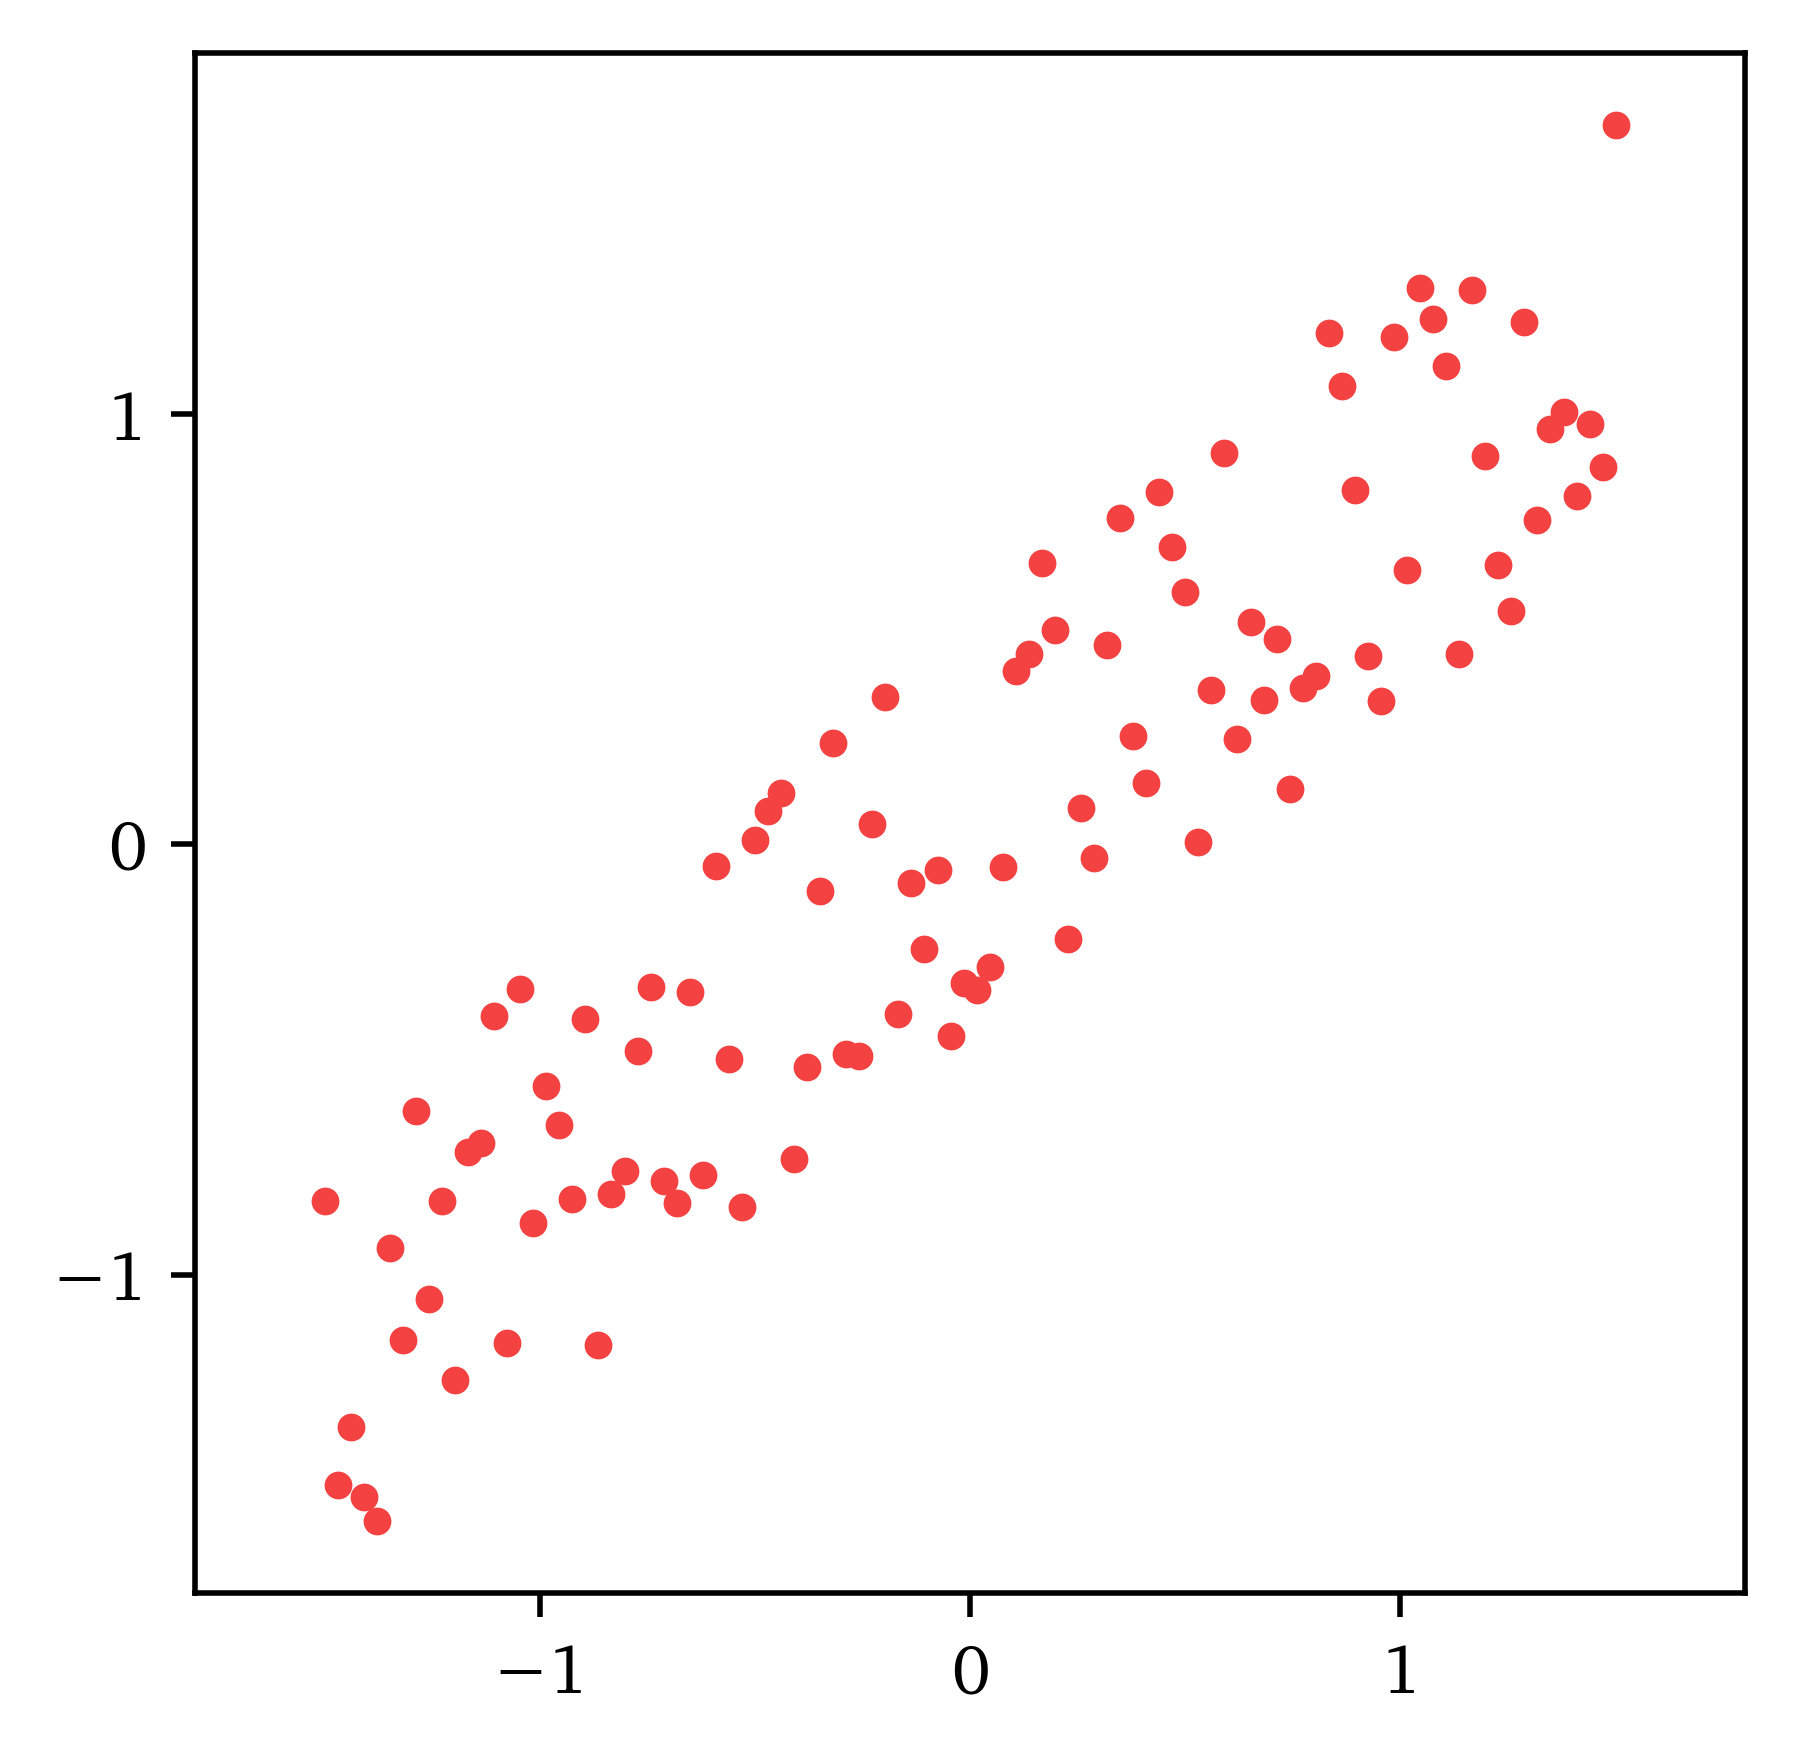
\includegraphics[width=7cm]{python-data-centered.png}
\caption{Dataset $\bm{X}$ centered.}
\label{fig:python-raw-data-centered}
\end{figure}

\begin{figure}[H]
\centering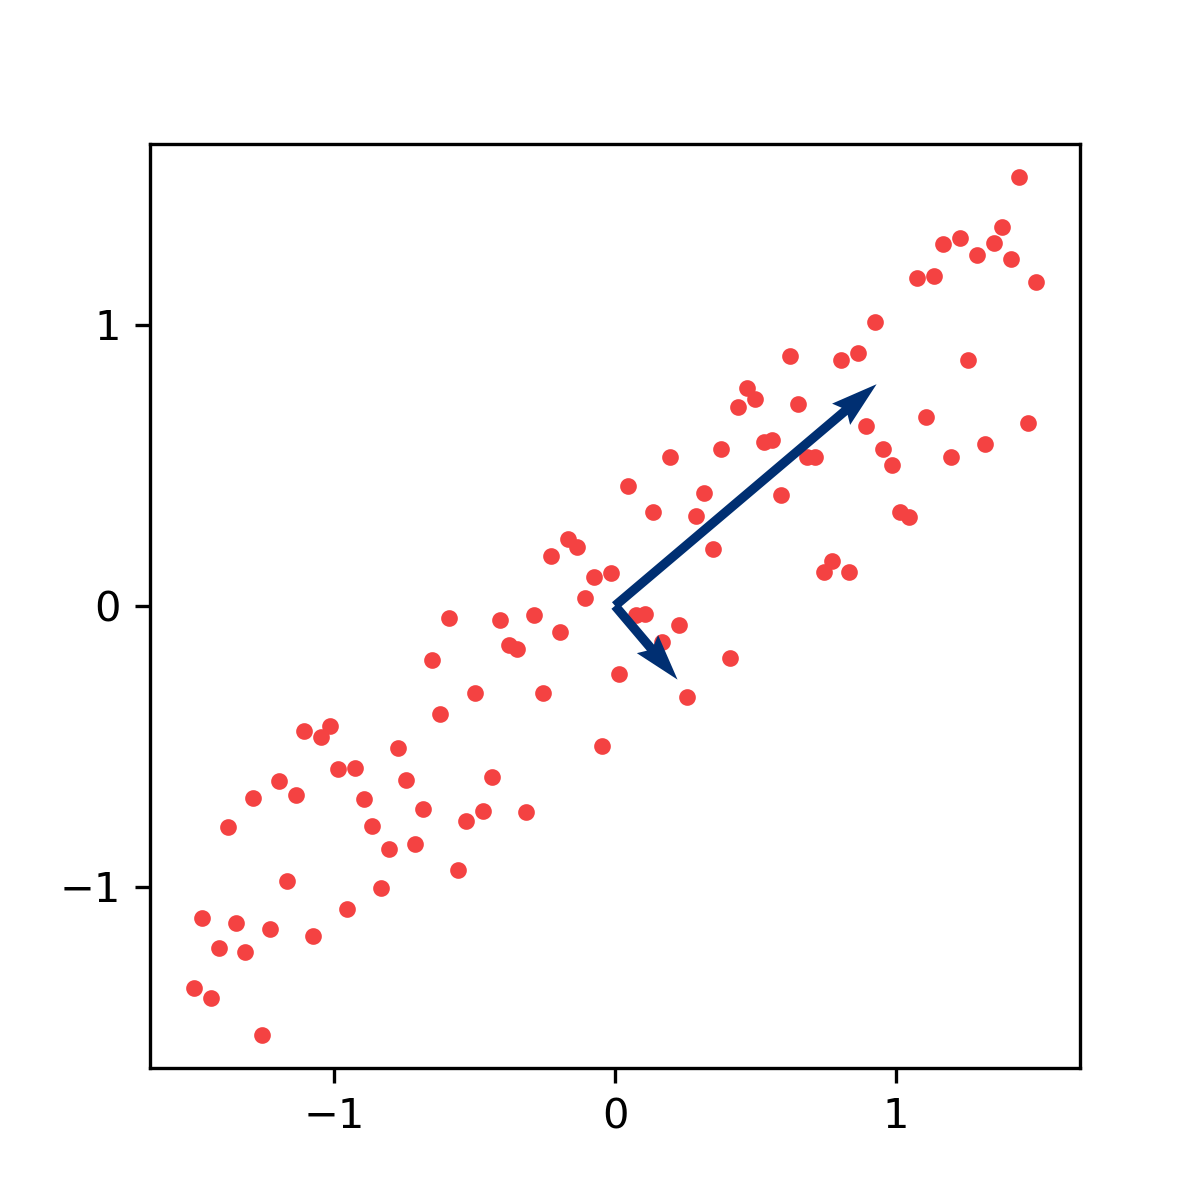
\includegraphics[width=7cm]{python-PCs.png}
\caption{Data set with principal components.}
\label{fig:python-PCs}
\end{figure}

\begin{figure}[H]
\centering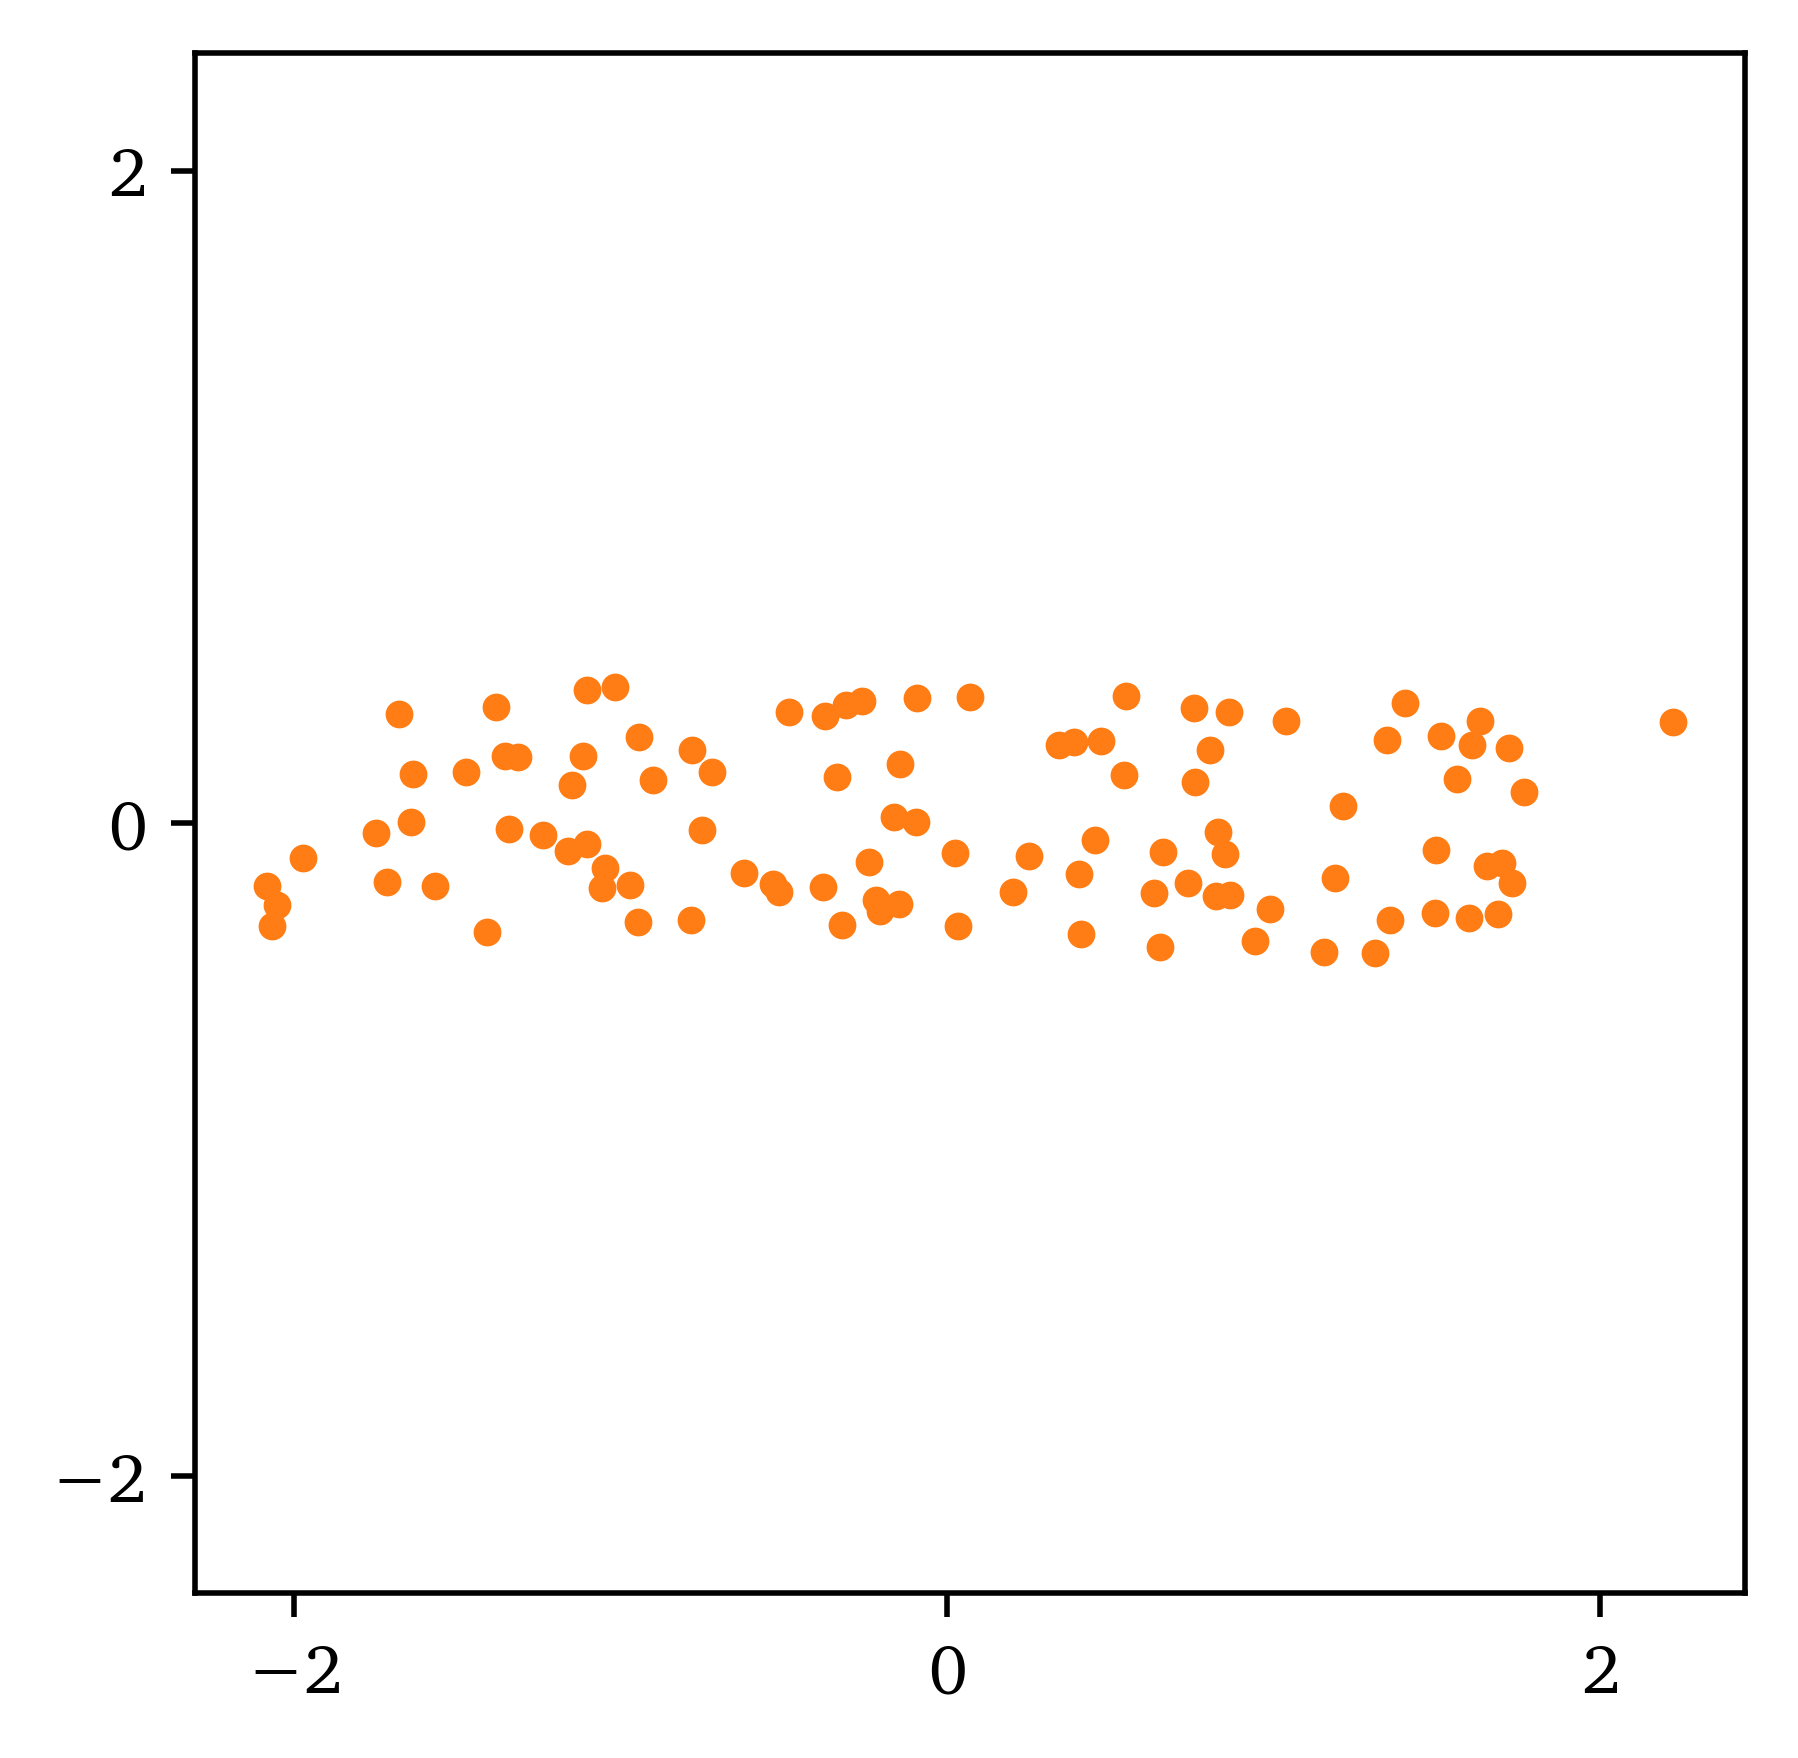
\includegraphics[width=7cm]{python-PC-scores.png}
\caption{PC-scores.}
\label{fig:python-PC-scores}
\end{figure}

\begin{figure}[H]
\centering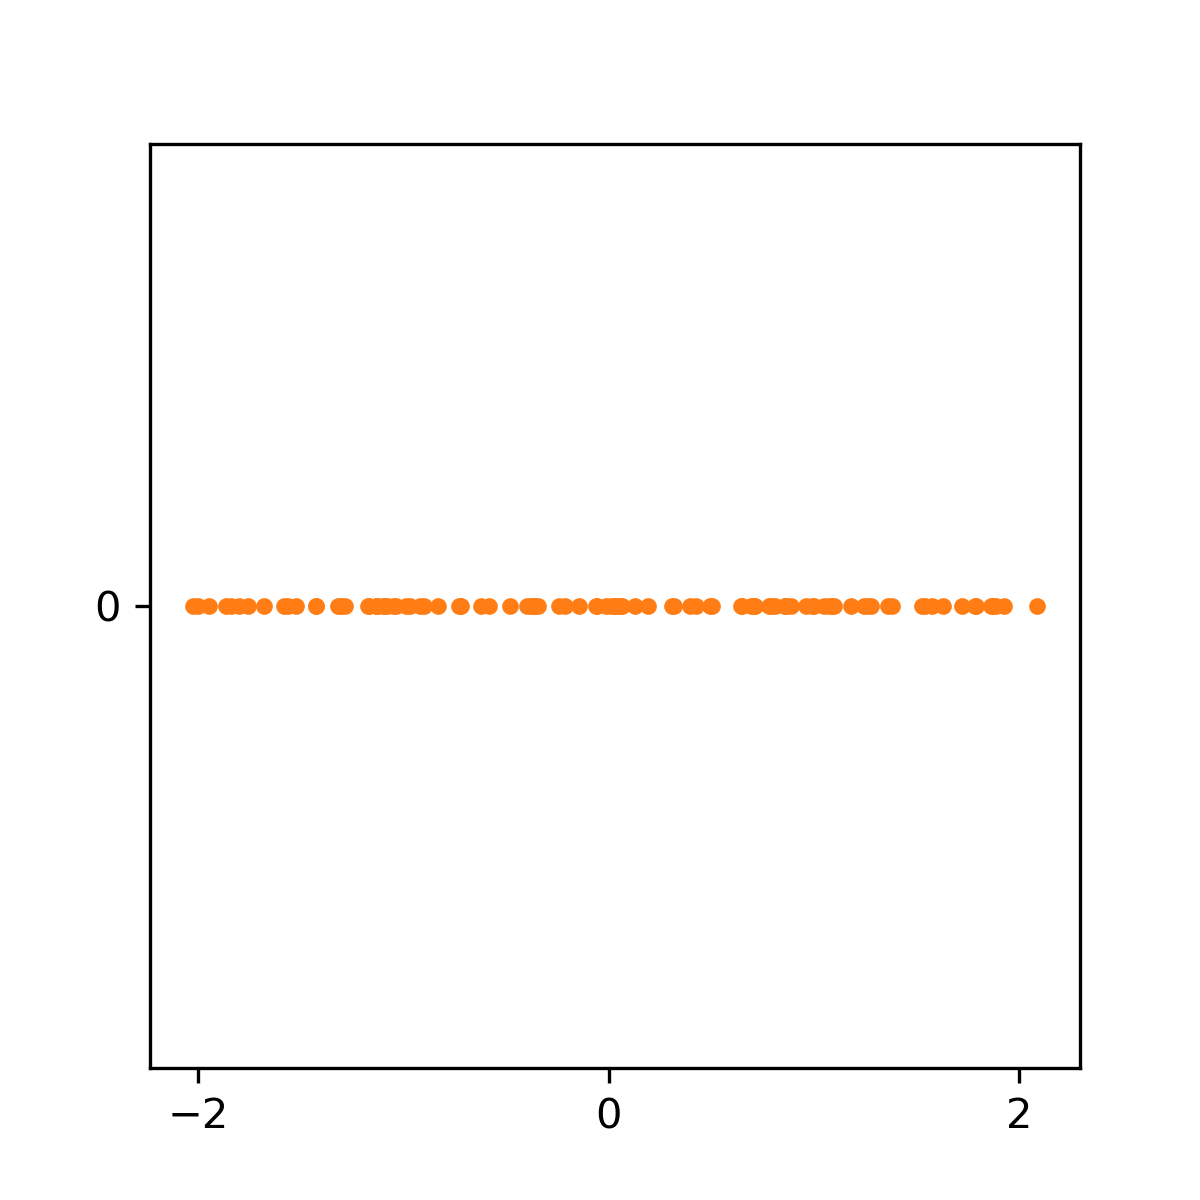
\includegraphics[width=7cm]{python-data-projection.png}
\caption{Data projection.}
\label{fig:python-data-projection}
\end{figure}

\begin{figure}[H]
\centering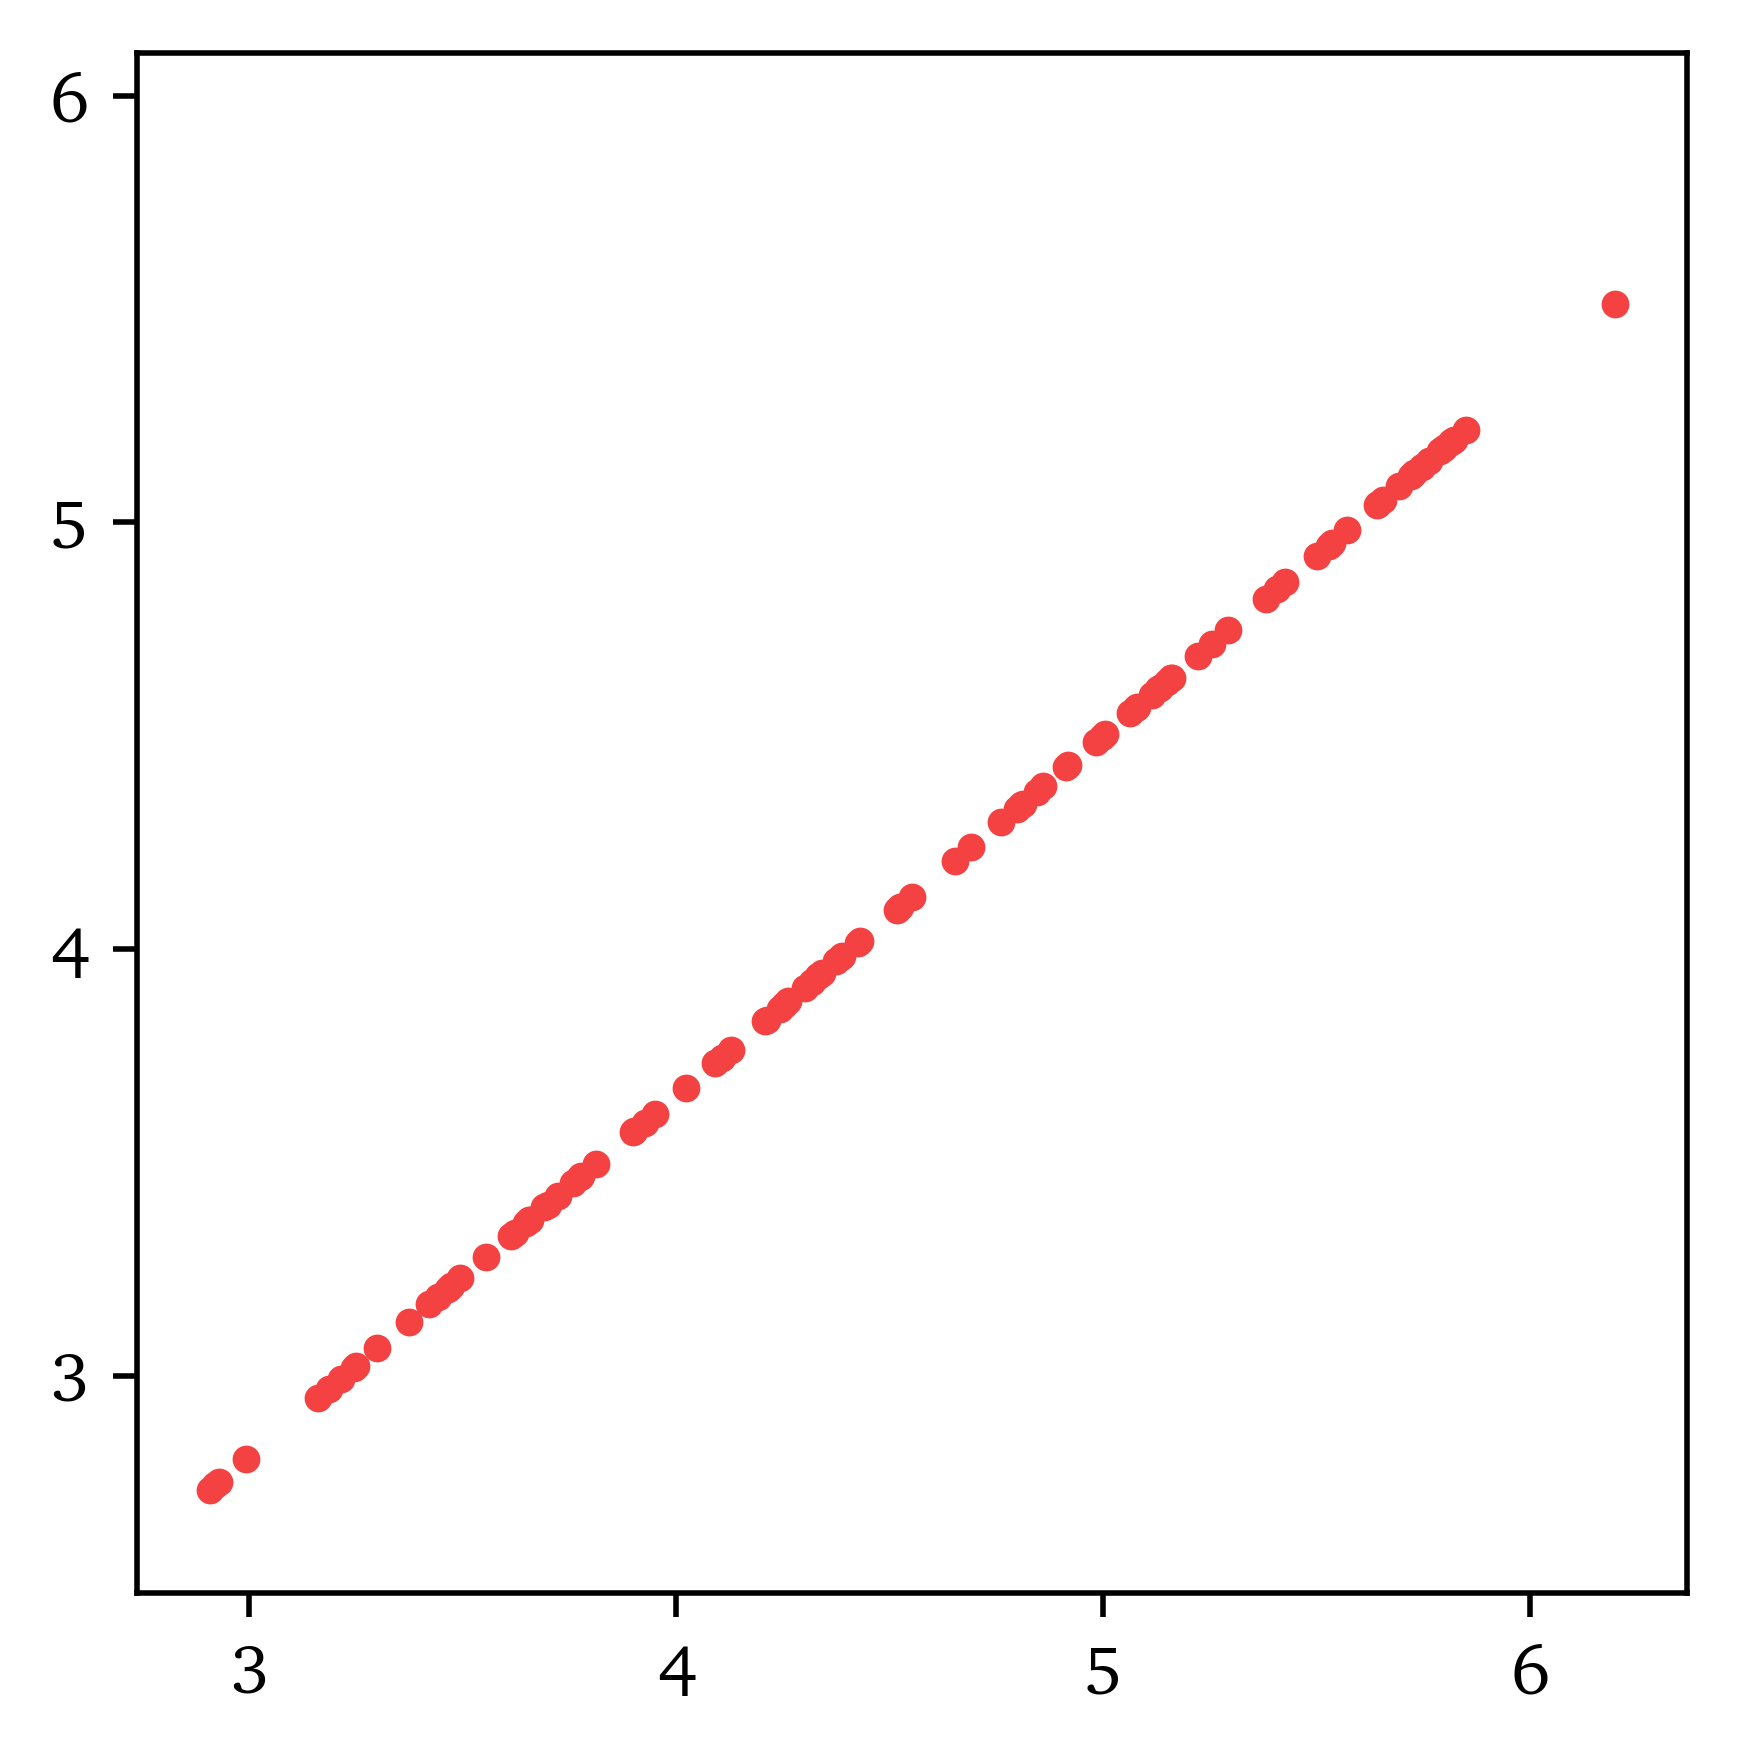
\includegraphics[width=7cm]{python-data-approximation.png}
\caption{Data approximation with $q = 1$.}
\label{fig:python-data-approximation}
\end{figure}

\section{Interesting questions}

Is the covariance matrix of PC-scores a diagonal matrix?

\appendix

\section{APP1} \label{app:A}

\section{APP2} \label{app:B}

\thebibliography{}

\bibitem{Matlab-pca} \texttt{https://nl.mathworks.com/help/stats/pca.html}
\bibitem{Jolliffe} Ian T. Jolliffe, \textit{Principal Component Analysis}, Second Edition, 1986
\bibitem{Strang} Gilbert Strang, \textit{Introduction to Linear Algebra}, Fifth Edition, 2016
\bibitem{Shlens} Jonathon Shlens, \textit{A Tutorial on Principal Component Analysis}, 2016, \texttt{https://arxiv.org/abs/1404.1100}
\bibitem{cov-dot} \texttt{http://people.sju.edu/~pklingsb/dot.cov.pdf}
\bibitem{Jackson} J. Edward Jackson, \textit{A User's Guide To Principal Components}, 1991
\bibitem{Smith} Lindsay I. Smith, \textit{A tutorial on Principal Component Analysis}, 2002

\end{document}
